\documentclass[12pt,a4paper,oneside]{book}

% Packages
\usepackage[utf8]{inputenc}
\usepackage[left=0.75in,right=0.75in,top=0.75in,bottom=1in]{geometry}
\usepackage{xcolor}
\usepackage{tikz}
\usetikzlibrary{shapes.geometric,shadows,patterns,positioning}
\usepackage{enumitem}
\usepackage{tcolorbox}
\usepackage{helvet}
\usepackage{setspace}
\usepackage{fancyhdr}
\usepackage{graphicx}
\usepackage{listings}
\usepackage{lstautogobble}

% Font settings
\renewcommand{\familydefault}{\sfdefault}
\setstretch{1.15}

% Define colors
\definecolor{headerred}{RGB}{213,43,30}
\definecolor{jsyellow}{RGB}{247,223,30}
\definecolor{cssblue}{RGB}{38,77,228}
\definecolor{htmlorange}{RGB}{228,77,38}
\definecolor{codebg}{RGB}{245,245,245}
\definecolor{codecomment}{RGB}{0,128,0}
\definecolor{codekeyword}{RGB}{0,0,255}
\definecolor{codestring}{RGB}{163,21,21}

% Listings settings for advanced look
\lstset{
    backgroundcolor=\color{codebg},
    basicstyle=\ttfamily\small,
    breaklines=true,
    frame=single,
    frameround=tttt,
    framexleftmargin=5pt,
    numbers=left,
    numberstyle=\tiny\color{gray},
    numbersep=8pt,
    showstringspaces=false,
    keywordstyle=\color{codekeyword}\bfseries,
    commentstyle=\color{codecomment}\itshape,
    stringstyle=\color{codestring},
    tabsize=2,
    autogobble=true,
    captionpos=t,
    xleftmargin=15pt,
    framexleftmargin=10pt,
    framexrightmargin=5pt,
    framextopmargin=5pt,
    framexbottommargin=5pt,
    rulecolor=\color{gray!30},
    aboveskip=15pt,
    belowskip=10pt
}

% JavaScript style
\lstdefinestyle{javascript}{
    language=Java,
    morekeywords={let, const, async, await, of, function, var, return, if, else, for, while, do, switch, case, break, continue, new, this, typeof, instanceof, true, false, null, undefined, class, extends, import, export, default, from, as, static, get, set, constructor, super, yield, promise, resolve, reject, then, catch, finally},
    morecomment=[l]{//},
    morecomment=[s]{/*}{*/},
    morestring=[b]',
    morestring=[b]",
    morestring=[b]`,
    keywordstyle=\color{blue!70!black}\bfseries,
    commentstyle=\color{green!50!black}\itshape,
    stringstyle=\color{orange!80!black},
    backgroundcolor=\color{blue!3},
    frame=shadowbox,
    rulesepcolor=\color{blue!20!gray!20},
    escapeinside={(*@}{@*)}
}

% Custom chapter command
\newcommand{\mychapter}[1]{%
    \clearpage
    \stepcounter{chapter}
    \vspace*{-1in}
    \begin{tcolorbox}[
        colback=headerred,
        coltext=white,
        boxrule=0pt,
        arc=0pt,
        outer arc=0pt,
        left=0pt,
        right=0pt,
        top=30pt,
        bottom=30pt,
        width=\textwidth,
        enlarge left by=-0.75in,
        enlarge right by=-0.75in,
        width=\paperwidth
    ]
        \centering
        \Huge\bfseries \thechapter.~#1
    \end{tcolorbox}
    \vspace{1em}
    \addcontentsline{toc}{chapter}{\protect\numberline{\thechapter}#1}
}

% Section formatting
\newcommand{\mysection}[1]{%
    \vspace{0.3em}
    {\large\bfseries\underline{#1}}
    \vspace{0.2em}
    \addcontentsline{toc}{section}{#1}
}

% Page styles
\pagestyle{fancy}
\fancyhf{}
\fancyhead[C]{Full Stack Development}
\fancyfoot[C]{\thepage}
\renewcommand{\headrulewidth}{0pt}
\renewcommand{\footrulewidth}{0pt}

\fancypagestyle{plain}{
    \fancyhf{}
    \fancyfoot[C]{\thepage}
}

% Custom itemize
\setlist[itemize]{
    topsep=0.2em,
    itemsep=0.2em,
    parsep=0pt,
    partopsep=0pt,
    leftmargin=2em,
    label=\textbullet
}

\begin{document}
\frontmatter

% Title Page
\thispagestyle{empty}
\begin{titlepage}
    \begin{tikzpicture}[remember picture,overlay]
        \fill[headerred!10] (current page.north west) rectangle (current page.south east);
        \draw[headerred!30, line width=1pt] 
            ([xshift=1cm,yshift=-1cm]current page.north west) 
            rectangle ([xshift=-1cm,yshift=1cm]current page.south east);
    \end{tikzpicture}
    
    \vspace*{1cm}
    
    \begin{center}
        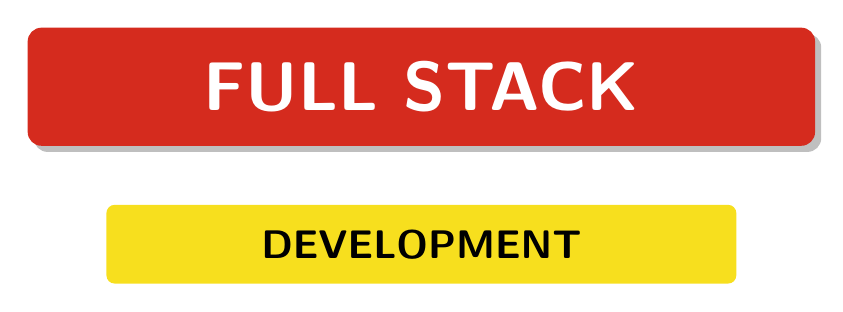
\begin{tikzpicture}
            \node[draw=none, fill=headerred, minimum width=10cm, minimum height=1.5cm, 
                  rounded corners=5pt, drop shadow] at (0,0) {
                \color{white}\Huge\bfseries FULL STACK
            };
            \node[draw=none, fill=jsyellow, 
                  minimum width=8cm, minimum height=1cm, rounded corners=3pt] at (0,-2) {
                \Large\bfseries DEVELOPMENT
            };
        \end{tikzpicture}
        
        \vspace{2cm}
        
        
\begin{tikzpicture}[scale=2]
            \node[draw=none, fill=jsyellow, minimum width=3cm, minimum height=3cm, 
                  rounded corners=5pt, drop shadow] at (0,0) {
                \Huge\bfseries\color{black} JS
            };
        \end{tikzpicture}
        
        \vspace{2cm}
        
        {\Large\color{headerred} JavaScript, Bootstrap, ReactJS \& MongoDB}\\[0.5cm]
        {\large Essential Concepts for Modern Web Development}\\[1.5cm]
        
        \vfill
        
        \begin{tcolorbox}[
            colback=white,
            coltext=black,
            boxrule=2pt,
            arc=5pt,
            width=10cm,
            center,
            colframe=headerred
        ]
            \centering
            \large\bfseries Author: Rama Bhadra Rao Maddu\\[0.3cm]
            \small Version 1.0 | \today
        \end{tcolorbox}
    \end{center}
\end{titlepage}

% Copyright Page
\clearpage
\thispagestyle{empty}
\vspace*{3cm}
\begin{center}
    \large\bfseries Copyright Notice
\end{center}

\vspace{1cm}

© 2024 Rama Bhadra Rao Maddu. All Rights Reserved.

\vspace{1cm}

\textbf{Publisher:} Self Published\\
\textbf{Author:} Rama Bhadra Rao Maddu\\
\textbf{First Edition:} 2024

\vfill

% Book Objectives
\clearpage
\thispagestyle{empty}
\vspace*{2cm}
\begin{center}
    \large\bfseries Book Objectives
\end{center}

\vspace{1cm}

The main objective of this course is to provide comprehensive understanding on:

\begin{itemize}
    \item Essential JavaScript concepts for web development
    \item Bootstrap framework for responsive design
    \item ReactJS for building modern user interfaces
    \item MongoDB for NoSQL database management
    \item Full-stack application development workflow
\end{itemize}

This book bridges the gap between frontend and backend development, enabling readers to build complete web applications from scratch.

% Table of Contents
\clearpage
\tableofcontents

\mainmatter
\setcounter{chapter}{0}

% CHAPTER 1 - BASIC JAVASCRIPT
\mychapter{BASIC JAVASCRIPT}

\mysection{Introduction to JavaScript}

JavaScript is a high-level, interpreted programming language that has become one of the core technologies of the World Wide Web. Created by Brendan Eich in 1995 in just 10 days at Netscape Communications, JavaScript has evolved from a simple scripting language to power complex web applications, server-side development through Node.js (created by Ryan Dahl in 2009), and even mobile applications.

\textbf{Key Characteristics of JavaScript:}
\begin{itemize}
    \item \textbf{Dynamic Typing:} Variables can hold values of any type without declaring the type
    \item \textbf{Interpreted:} No compilation step required; code is executed directly
    \item \textbf{Prototype-based:} Objects can inherit directly from other objects
    \item \textbf{First-class Functions:} Functions are treated as values
    \item \textbf{Event-driven:} Responds to user interactions and system events
    \item \textbf{Multi-paradigm:} Supports procedural, object-oriented, and functional programming
\end{itemize}

\textbf{JavaScript Engines:}

JavaScript code is executed by JavaScript engines. Each browser uses a different engine:
\begin{itemize}
    \item \textbf{V8:} Used by Google Chrome and Node.js (developed by Google)
    \item \textbf{SpiderMonkey:} Used by Mozilla Firefox
    \item \textbf{JavaScriptCore:} Used by Safari (Apple)
    \item \textbf{Chakra:} Used by Internet Explorer and Legacy Microsoft Edge
\end{itemize}

\textbf{Client-side vs Server-side JavaScript:}

\begin{itemize}
    \item \textbf{Client-side (Browser):} 
    \begin{itemize}
        \item Runs in web browsers
        \item Manipulates DOM
        \item Handles user interactions
        \item Makes AJAX requests
        \item Has access to browser APIs
        \item Restricted file system access for security
    \end{itemize}
    
    \item \textbf{Server-side (Node.js):}
    \begin{itemize}
        \item Runs on servers
        \item Full file system access
        \item Can connect to databases
        \item Creates HTTP servers
        \item No DOM access
        \item Can use npm packages
    \end{itemize}
\end{itemize}

\mysection{JavaScript Instructions and Statements}

A JavaScript program is a list of programming statements or instructions. Each statement performs a specific action and ends with a semicolon (though semicolons are optional in many cases due to automatic semicolon insertion).

\begin{lstlisting}[style=javascript, caption={\textbf{Basic JavaScript Statements}}, label=lst:statements]
// A simple statement
console.log("Hello, World!");

// Multiple statements
let message = "Learning JavaScript";
console.log(message);

// Statements can span multiple lines
let longMessage = "This is a very long message that " +
                  "spans multiple lines for readability";

// Compound statement (block)
{
    let x = 5;
    let y = 10;
    console.log(x + y);
}

// Statement types examples
let declaration = "This is a declaration statement";
5 + 3; // Expression statement
if (true) { /* Control flow statement */ }
function example() { return; } // Jump statement
\end{lstlisting}

\textbf{Statement Types:}
\begin{itemize}
    \item \textbf{Expression statements:} Evaluate to a value
    \item \textbf{Declaration statements:} Declare variables or functions
    \item \textbf{Control flow statements:} Control program execution
    \item \textbf{Jump statements:} Transfer control
\end{itemize}

\mysection{Comments in JavaScript}

Comments are essential for code documentation and are ignored by the JavaScript engine during execution.

\begin{lstlisting}[style=javascript, caption={\textbf{Types of Comments in JavaScript}}, label=lst:comments]
// Single-line comment
// This explains what the next line does
let userName = "John";

/* 
   Multi-line comment
   This is useful for longer explanations
   or temporarily disabling code blocks
*/

let age = 25; // Inline comment

/** 
 * JSDoc comment for documentation
 * @param {string} name - The user's name
 * @param {number} age - The user's age
 * @returns {string} A greeting message
 */
function createGreeting(name, age) {
    return `Hello ${name}, you are ${age} years old`;
}

// TODO: Add validation
// FIXME: Handle edge cases
// NOTE: This is deprecated
\end{lstlisting}

\mysection{Variables in JavaScript}

Variables are containers for storing data values. JavaScript has evolved from using only \texttt{var} to modern \texttt{let} and \texttt{const} declarations.

\subsubsection{Variable Declaration Keywords}

\begin{lstlisting}[style=javascript, caption={\textbf{Variable Declaration Methods - var, let, const}}, label=lst:variables]
// var - Function-scoped (ES5 and earlier)
var oldVariable = "I'm function-scoped";
var canBeRedeclared = "first";
var canBeRedeclared = "second"; // Allowed

// let - Block-scoped (ES6+)
let modernVariable = "I'm block-scoped";
let cannotBeRedeclared = "only once";
// let cannotBeRedeclared = "error"; // SyntaxError

// const - Block-scoped, cannot be reassigned (ES6+)
const constantVariable = "I cannot be reassigned";
// constantVariable = "new value"; // TypeError

// const with objects and arrays
const person = { name: "John" };
person.name = "Jane"; // Allowed - modifying property
// person = { name: "Bob" }; // Error - reassigning

const numbers = [1, 2, 3];
numbers.push(4); // Allowed - modifying array
// numbers = [5, 6, 7]; // Error - reassigning
\end{lstlisting}

\subsubsection{Variable Scope}

\begin{lstlisting}[style=javascript, caption={\textbf{Understanding Variable Scope}}, label=lst:scope]
// Global scope
var globalVar = "I'm global";
let globalLet = "I'm also global";

function demonstrateScope() {
    // Function scope
    var functionScoped = "Available throughout function";
    
    if (true) {
        // Block scope
        var varInBlock = "Still function-scoped";
        let letInBlock = "Only in this block";
        const constInBlock = "Also only in this block";
        
        console.log(functionScoped); // Works
        console.log(varInBlock);     // Works
        console.log(letInBlock);     // Works
    }
    
    console.log(functionScoped); // Works
    console.log(varInBlock);     // Works (var ignores block)
    // console.log(letInBlock);  // ReferenceError
    // console.log(constInBlock); // ReferenceError
}
\end{lstlisting}

\subsubsection{Hoisting}

Hoisting is JavaScript's default behavior of moving declarations to the top of their scope before code execution.

\begin{lstlisting}[style=javascript, caption={\textbf{Understanding Hoisting with var, let, and const}}, label=lst:hoisting]
// Hoisting with var
console.log(hoistedVar); // undefined (not error)
var hoistedVar = "I'm hoisted";
console.log(hoistedVar); // "I'm hoisted"

// The above is interpreted as:
// var hoistedVar; // Declaration hoisted
// console.log(hoistedVar); // undefined
// hoistedVar = "I'm hoisted"; // Assignment stays

// Hoisting with let/const (Temporal Dead Zone)
// console.log(notAccessible); // ReferenceError
let notAccessible = "I'm in the TDZ";

// Function hoisting
console.log(myFunction()); // "Works!"
function myFunction() {
    return "Works!";
}

// Function expressions are not hoisted
// console.log(myExpression()); // TypeError
var myExpression = function() {
    return "Not hoisted";
};

// Temporal Dead Zone (TDZ) demonstration
function demonstrateTDZ() {
    // TDZ starts for 'temp'
    // console.log(temp); // ReferenceError
    let temp = "Now accessible"; // TDZ ends
    console.log(temp); // "Now accessible"
}
\end{lstlisting}

\mysection{Data Types in JavaScript}

JavaScript is dynamically typed with seven primitive types and one non-primitive type (Object).

\subsubsection{Primitive Data Types}

\begin{lstlisting}[style=javascript, caption={\textbf{All Primitive Data Types}}, label=lst:datatypes]
// 1. Number - Integers and floating-point
let integer = 42;
let float = 3.14159;
let exponential = 2.5e3;  // 2500
let hexadecimal = 0xFF;   // 255
let binary = 0b1010;      // 10
let octal = 0o12;         // 10

// Special numeric values
let infinity = Infinity;
let notANumber = NaN;

// 2. String - Text data
let singleQuote = 'Hello';
let doubleQuote = "World";
let templateLiteral = `Hello ${doubleQuote}`;

// 3. Boolean
let isTrue = true;
let isFalse = false;

// 4. Undefined
let undefinedVar;
console.log(undefinedVar); // undefined

// 5. Null
let nullVar = null;

// 6. Symbol (ES6)
let sym1 = Symbol('id');
let sym2 = Symbol('id');
console.log(sym1 === sym2); // false

// 7. BigInt (ES2020)
let bigInteger = 123n;
let bigFromString = BigInt("9007199254740992");
\end{lstlisting}

\subsubsection{Type Conversion and Coercion}

\begin{lstlisting}[style=javascript, caption={\textbf{Type Conversion and Coercion}}, label=lst:typeconversion]
// Explicit Conversion
let num = 123;
let str = String(num);        // "123"
let strToNum = Number("456"); // 456
let bool = Boolean(1);        // true

// Implicit Coercion
console.log("5" + 3);    // "53" (string)
console.log("5" - 3);    // 2 (number)
console.log(true + 1);   // 2

// Falsy values
// false, 0, -0, 0n, "", null, undefined, NaN

// Equality comparisons
console.log(5 == "5");   // true (coercion)
console.log(5 === "5");  // false (strict)
\end{lstlisting}

\mysection{Arrays in JavaScript}

Arrays are ordered collections that can hold multiple values of any type.

\subsubsection{Array Creation and Methods}

\begin{lstlisting}[style=javascript, caption={\textbf{Arrays - Creation and Methods}}, label=lst:arrays]
// Creating arrays
let numbers = [1, 2, 3, 4, 5];
let mixed = [1, "two", true, null];

// Accessing elements
console.log(numbers[0]);    // 1
console.log(numbers.length); // 5

// Mutating methods
numbers.push(6);        // Add to end
numbers.pop();          // Remove from end
numbers.unshift(0);     // Add to start
numbers.shift();        // Remove from start
numbers.splice(2, 1);   // Remove at index
numbers.sort();         // Sort in place
numbers.reverse();      // Reverse in place

// Non-mutating methods
let subset = numbers.slice(1, 3);
let joined = numbers.join("-");
let index = numbers.indexOf(3);

// Iteration methods (ES5+)
let doubled = numbers.map(n => n * 2);
let evens = numbers.filter(n => n % 2 === 0);
let sum = numbers.reduce((acc, n) => acc + n, 0);
let found = numbers.find(n => n > 3);

numbers.forEach((num, index) => {
    console.log(`Index ${index}: ${num}`);
});
\end{lstlisting}

\mysection{Strings in JavaScript}

Strings represent text data and are immutable.

\begin{lstlisting}[style=javascript, caption={\textbf{String Creation and Methods}}, label=lst:strings]
// Creating strings
let single = 'Single quotes';
let double = "Double quotes";
let template = `Template literal with ${double}`;

// String methods
let text = "  JavaScript  ";
console.log(text.length);           // 14
console.log(text.trim());           // "JavaScript"
console.log(text.toUpperCase());    // "  JAVASCRIPT  "
console.log(text.toLowerCase());    // "  javascript  "

// Searching
let sentence = "The quick brown fox";
console.log(sentence.indexOf("quick"));    // 4
console.log(sentence.includes("fox"));     // true
console.log(sentence.startsWith("The"));   // true

// Extracting
console.log(sentence.substring(4, 9));  // "quick"
console.log(sentence.slice(-3));        // "fox"

// Modifying (returns new string)
console.log(sentence.replace("fox", "dog"));
console.log(sentence.split(" ")); // Array of words
\end{lstlisting}

\mysection{Functions in JavaScript}

Functions are reusable blocks of code that perform specific tasks.

\begin{lstlisting}[style=javascript, caption={\textbf{Function Types and Features}}, label=lst:functions]
// Function Declaration (hoisted)
function greet(name) {
    return "Hello, " + name;
}

// Function Expression
const multiply = function(a, b) {
    return a * b;
};

// Arrow Function (ES6)
const square = x => x * x;
const sum = (a, b) => a + b;

// Default parameters (ES6)
function greetWithDefault(name = "World") {
    return `Hello, ${name}!`;
}

// Rest parameters (ES6)
function sumAll(...numbers) {
    return numbers.reduce((acc, n) => acc + n, 0);
}

// Destructuring parameters
function createUser({name, age, email = "N/A"}) {
    return { name, age, email, id: Date.now() };
}

// Closures
function createCounter(start = 0) {
    let count = start;
    return {
        increment: () => ++count,
        decrement: () => --count,
        getValue: () => count
    };
}

// Higher-order function
function withLogging(fn) {
    return function(...args) {
        console.log(`Calling with: ${args}`);
        return fn(...args);
    };
}

// IIFE (Immediately Invoked Function Expression)
(function() {
    console.log("IIFE executed!");
})();
\end{lstlisting}

\mysection{Objects and Methods}

Objects are collections of key-value pairs.

\begin{lstlisting}[style=javascript, caption={\textbf{Objects - Creation and Manipulation}}, label=lst:objects]
// Object literal
const person = {
    firstName: "John",
    lastName: "Doe",
    age: 30,
    
    // Method
    getFullName() {
        return `${this.firstName} ${this.lastName}`;
    }
};

// Accessing properties
console.log(person.firstName);      // Dot notation
console.log(person["lastName"]);    // Bracket notation
console.log(person.getFullName());  // Method call

// Adding/modifying properties
person.email = "john@example.com";
person.age = 31;

// Deleting properties
delete person.email;

// Object methods
console.log(Object.keys(person));   // Array of keys
console.log(Object.values(person)); // Array of values
console.log(Object.entries(person)); // Array of [key, value]

// Object destructuring
const { firstName, age } = person;

// Spread operator
const copied = { ...person };
const merged = { ...person, city: "NYC" };

// Constructor function
function Car(make, model, year) {
    this.make = make;
    this.model = model;
    this.year = year;
}

const myCar = new Car("Toyota", "Camry", 2022);

// ES6 Class
class Animal {
    constructor(name) {
        this.name = name;
    }
    
    speak() {
        return `${this.name} makes a sound`;
    }
}

const dog = new Animal("Buddy");
\end{lstlisting}

\mysection{Decisions and Loops}

Control flow statements control the execution path of your program.

\subsubsection{Conditional Statements}

\begin{lstlisting}[style=javascript, caption={\textbf{Decision Making Structures}}, label=lst:decisions]
// if...else
let age = 18;
if (age < 18) {
    console.log("Minor");
} else if (age < 65) {
    console.log("Adult");
} else {
    console.log("Senior");
}

// switch
let day = 1;
switch (day) {
    case 0:
        console.log("Sunday");
        break;
    case 1:
        console.log("Monday");
        break;
    default:
        console.log("Other day");
}

// Ternary operator
let status = age >= 18 ? "adult" : "minor";

// Nullish coalescing (ES2020)
let username = null;
let displayName = username ?? "Guest";

// Optional chaining (ES2020)
let user = { profile: { name: "Alice" } };
console.log(user?.profile?.name); // "Alice"
console.log(user?.settings?.theme); // undefined
\end{lstlisting}

\subsubsection{Loops}

\begin{lstlisting}[style=javascript, caption={\textbf{Loop Structures}}, label=lst:loops]
// for loop
for (let i = 0; i < 5; i++) {
    console.log(i);
}

// while loop
let count = 0;
while (count < 5) {
    console.log(count);
    count++;
}

// do...while loop
let num = 0;
do {
    console.log(num);
    num++;
} while (num < 3);

// for...in (objects)
const obj = { a: 1, b: 2, c: 3 };
for (let key in obj) {
    console.log(`${key}: ${obj[key]}`);
}

// for...of (iterables)
const arr = [1, 2, 3];
for (let value of arr) {
    console.log(value);
}

// break and continue
for (let i = 0; i < 10; i++) {
    if (i === 5) break;     // Exit loop
    if (i % 2 === 0) continue; // Skip iteration
    console.log(i);
}

// Array iteration methods
[1, 2, 3].forEach(n => console.log(n));
let doubled = [1, 2, 3].map(n => n * 2);
let evens = [1, 2, 3, 4].filter(n => n % 2 === 0);
let sum = [1, 2, 3].reduce((acc, n) => acc + n, 0);
\end{lstlisting}

% Future chapters placeholder
\chapter{DOM MANIPULATION}
\textit{This chapter will cover Document Object Model manipulation...}

\chapter{FORMS AND REACT INTRODUCTION}
\textit{This chapter will cover HTML forms and introduction to React...}

\chapter{REACT STATE AND APIs}
\textit{This chapter will cover React state management and API integration...}

\chapter{MONGODB AND WEBPACK}
\textit{This chapter will cover MongoDB NoSQL database and Webpack bundling...}

\end{document}